% Created 2014-12-11 Thu 13:35
\documentclass[9pt,b5paper]{article}
\usepackage{graphicx}
\usepackage{xcolor}
\usepackage{xeCJK}
\usepackage{longtable}
\usepackage{float}
\usepackage{textcomp}
\usepackage{geometry}
\geometry{left=0cm,right=0cm,top=0cm,bottom=0cm}
\usepackage{multirow}
\usepackage{multicol}
\usepackage{listings}
\usepackage{algorithm}
\usepackage{algorithmic}
\usepackage{latexsym}
\usepackage{natbib}
\usepackage{fancyhdr}
\usepackage[xetex,colorlinks=true,CJKbookmarks=true,linkcolor=blue,urlcolor=blue,menucolor=blue]{hyperref}


\lstset{language=c++,numbers=left,numberstyle=\tiny,basicstyle=\ttfamily\small,tabsize=4,frame=none,escapeinside=``,extendedchars=false,keywordstyle=\color{blue!70},commentstyle=\color{red!55!green!55!blue!55!},rulesepcolor=\color{red!20!green!20!blue!20!}}
\author{Heyan Huang}
\date{\today}
\title{MIDI Command Controller Interface}
\hypersetup{
  pdfkeywords={},
  pdfsubject={},
  pdfcreator={Emacs 24.3.1 (Org mode 8.2.7c)}}
\begin{document}

\maketitle
\tableofcontents


\section{Update 12/11/2014, updates include}
\label{sec-1}
\begin{itemize}
\item Temporatorily mimic phonon seekslider, but have not connected the signals and slots fully functioning yet;
\item This seekslider may still eventually came back to use Phonon library using Qt4.8 version;
\item So far consider this as a bonux feature;
\end{itemize}
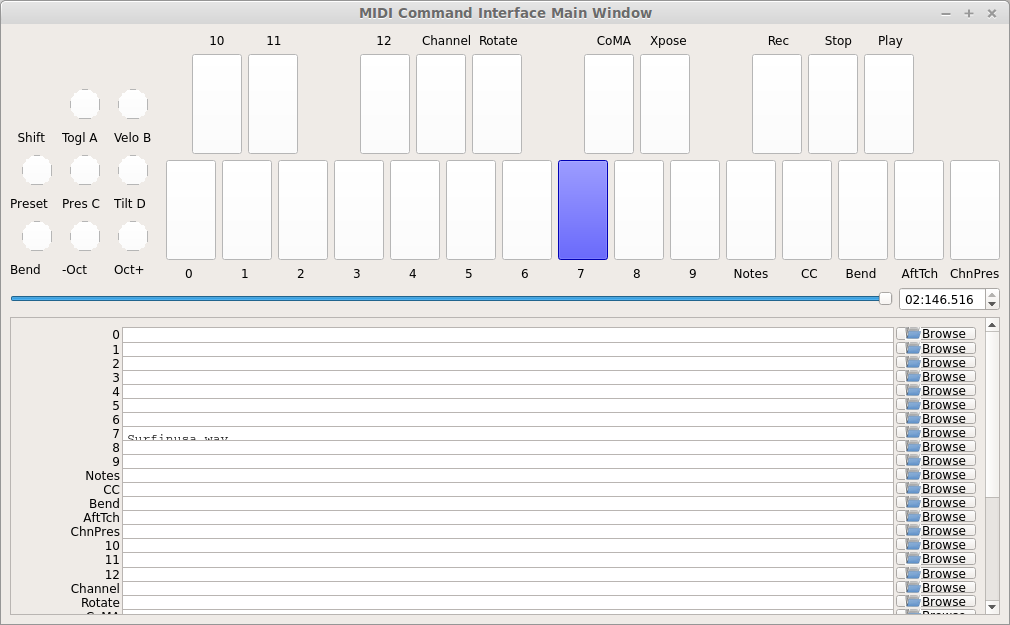
\includegraphics[width=.9\linewidth]{./pic/Screenshot_from_2014-12-11_13:33:46.png}

\section{Update 12/09/2014, updates include}
\label{sec-2}
\begin{itemize}
\item worked in it a little bit to set the connections between Midi controller and Qt Creator;
\item tried to implement pthead for reading user input, but got slightly frustrated today, and applied easier methods instead;
\item the project basically satisfied the instructor's requirements for connecting one key to work for playing his sequence, for example, Surfinusa.wav file;
\item Will demo to his to see if he has better suggestions.
\end{itemize}

\section{Update 11/23/2014, updates include}
\label{sec-3}
\begin{itemize}
\item Cleaned repository so that it looks clean and nice;
\item Remove menubar as suggested by advisor;
\item Removed topright four line texts cause it's not necessary;
\item Shifted top line keys so that they look like original midi controller layout;
\item Changed PlainTextEdit so that they satifies the requirements;
\item Added left side 8 keys, just that three keys \textbf{Bend}, \textbf{-Oct}, \textbf{Oct+} are \textbf{NOT} like the original shapes yet, need work on them later on;
\item Will link possible functionalities to make it a functional softwares first, and then updates minus issues.
\item Current layout looks as below snapshotted:
\end{itemize}

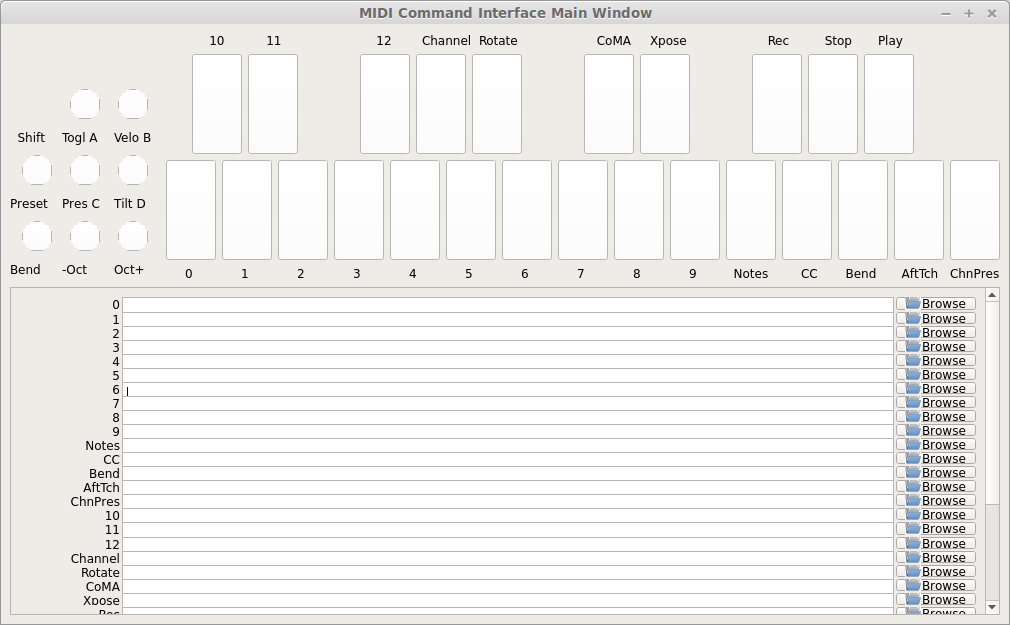
\includegraphics[width=.9\linewidth]{./pic/Screenshot_from_2014-11-23_13:20:06.png}  

\section{Review 11/21/2014, updates include}
\label{sec-4}
\subsection{Review Contents}
\label{sec-4-1}
\begin{itemize}
\item Created most basic interface for the client, and reviewed with course instructor.
\item Demo the most basic interface to him, and get corresponding specific requirements as listed followed.
\end{itemize}

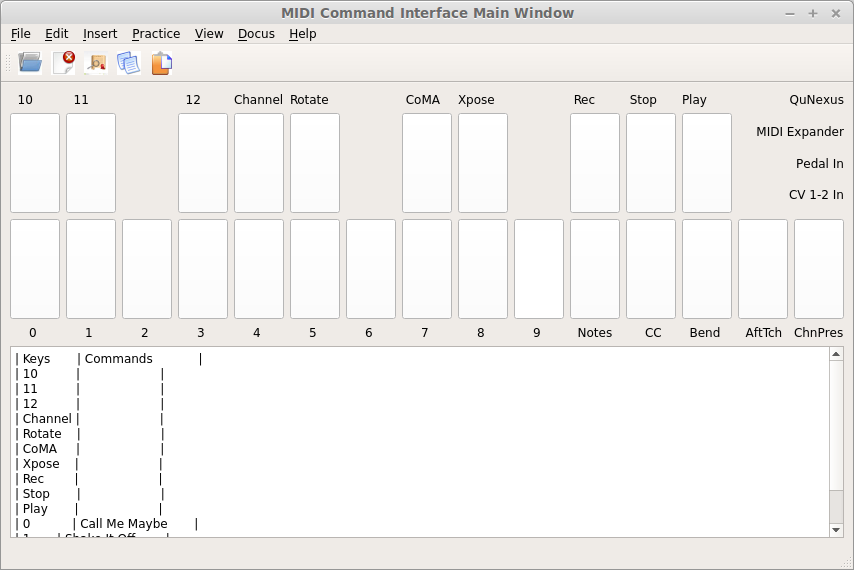
\includegraphics[width=.9\linewidth]{./pic/2014-11-20_21:52:19.png}

\subsection{Detailed Requirements}
\label{sec-4-2}
\begin{itemize}
\item menubar is NOT necessary, and could be removed away;
\item Interface topright four line texts are not necessary, could be removed away;
\item Interface top line keys should shift to the right by half key width so that the interface looks similar to the original midi controller keyboard;
\item PlainTextEdit should be changed to be array of 25/33 lines of (text label, file name editor, browse QPushButton keys) layout;
\item Left handside 8 keys should be included in the midi interface even functionalities are not required at this moment;
\item When finished the above basic ones, if I have extra time, could explore the left side 8 keys to test if it is possible to use them to set a bunch of sequence so that save time when needed compared with set sequence one by one from the basic 25 keys.
\end{itemize}

\section{Project Requirements}
\label{sec-5}
\begin{itemize}
\item Use QuNexus Midi controller as a command controller to manipulate play sequence for tower lights show;
\item Besides the main functionalities, create a Qt Creator Interface to help facilate the tower light playing process for clients convenience.
\end{itemize}

\section{main functionality}
\label{sec-6}
\subsection{Read data from MIDI}
\label{sec-6-1}
\begin{itemize}
\item Use the MIDI Controller as a speical Controller that can be operated to play specific songs sequence, or do some specific work.
\item play specific sequence may be the work for keys 0-9, and 10-12, how about other 20 keys? Do they require specific work to be done?
\end{itemize}
\subsection{Write data back to MIDI}
\label{sec-6-2}
\begin{itemize}
\item When a key was pushed, the specific Controller key's LED is supposed to be on to indicate the operation.
\item Trick about the LED to be continuously on is that when a key is pressed, that is 1 byte that indicates the "Duration" of the key press, I may need to 
\begin{itemize}
\item try to set this byte to be a large value, (1 byte, 2$^{\text{8}}$ = 256, it has limits!)
\item or continuously reset is to be that large value;
\item or continuously write this key to be pressed data back to MIDI with time intervals
\end{itemize}
\end{itemize}

\section{Programming Language}
\label{sec-7}
\subsection{Qt}
\label{sec-7-1}
\begin{itemize}
\item the worries that I have by using Qt is that if Qt has the capability to handle the MIDI-Linux connection problems.
\item And also Qt-to-Audio (linux) connection things as well. Should it be Qt, or as far as I can set it to work in Linux, just let it be that way then?
\end{itemize}
\subsection{c++}
\label{sec-7-2}
\begin{itemize}
\item I believe C++ is the most widely used Language used by those midi sequencer softwares, so I have no better choice than c++ right now.
\end{itemize}

\section{Interface Design}
\label{sec-8}
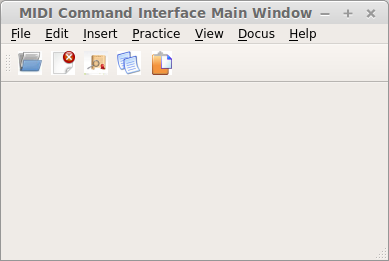
\includegraphics[width=.9\linewidth]{./pic/menu.png}

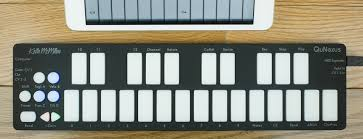
\includegraphics[width=.9\linewidth]{./pic/midi.jpg}

\section{Midi keys and corresponded operations}
\label{sec-9}
\begin{table}[htb]
\caption{midi keys and corresponded operations}
\centering
\begin{tabular}{ll}
\hline
Keys & Commands\\
\hline
10 & \\
11 & \\
12 & \\
channel & \\
Rotate & \\
CoMA & \\
Xpose & \\
Rec & \\
Stop & \\
Play & \\
\hline
0 & Call Me Maybe\\
1 & Shake It Off\\
2 & All About That Bass\\
3 & \ldots{}\\
4 & \\
5 & \\
6 & \\
7 & \\
8 & \\
9 & \\
\hline
Notes: & \\
CC & \\
Bend & \\
AftTch & \\
ChnPres & \\
\hline
Togl A & \\
Velo B & \\
Preset & \\
Pres C & \\
Tilt D & \\
Bend & \\
Oct- & \\
Oct+ & \\
\hline
\end{tabular}
\end{table}

\section{Interface Guide}
\label{sec-10}
\begin{itemize}
\item Give text instructions on how to use the Interface, and what are the corresponded operations by press specific keys.
\item Like list the above table in the Interface Guide text area.
\end{itemize}

\section{References}
\label{sec-11}
\begin{itemize}
\item For circle QPushButton
\begin{itemize}
\item \url{http://stackoverflow.com/questions/12734319/change-rectangular-qt-button-to-round}
\end{itemize}
\item Draw circle separate
\begin{itemize}
\item \url{https://coderalbert.wordpress.com/2014/03/16/creating-circle-in-linux-using-qt-creator/}
\end{itemize}
\item For Rectangle Arc
\begin{itemize}
\item \url{http://stackoverflow.com/questions/20416789/how-to-add-a-small-triangle-at-one-of-the-corners-of-qwidget}
\end{itemize}
\item PaintEvent Triangle
\begin{itemize}
\item \url{http://stackoverflow.com/questions/20416789/how-to-add-a-small-triangle-at-one-of-the-corners-of-qwidget}
\item \url{http://stackoverflow.com/questions/3894737/qt4-how-to-draw-inside-a-widget}
\item \url{http://qt-project.org/forums/viewthread/1623}
\item \url{http://stackoverflow.com/questions/7968269/basic-qt-gui-qpushbutton-for-drawing-a-line}
\end{itemize}
\item QPushButton::drawButton(QPainter *painter);
\begin{itemize}
\item \url{https://www.tbi.univie.ac.at/~pmg/tutorials/QT/html/qpushbutton.html}
\end{itemize}
\item QGraphicsSene QGraphicsProxy\ldots{}
\begin{itemize}
\item \url{http://qt-project.org/forums/viewthread/4020}
\end{itemize}
\item QPushButton raised enabled
\begin{itemize}
\item \url{http://www.qtcentre.org/threads/42852-QStyledItemDelegate-paint-QPushButton-with-stylesheet}
\end{itemize}
\item QPushButton two icons
\begin{itemize}
\item \url{http://www.qtcentre.org/threads/39445-How-to-add-two-icons-images-to-the-same-QPushButton}
\end{itemize}
\item QPainter
\begin{itemize}
\item \url{http://qt-project.org/forums/viewthread/23628}
\end{itemize}
\item QGridLayout ScrollArea
\begin{itemize}
\item \url{http://qt-project.org/forums/viewthread/20843}
\item \url{http://qt-project.org/forums/viewthread/20924/}
\end{itemize}
\item Leftover five
\begin{itemize}
\item \url{http://qt-project.org/doc/qt-4.8/qpainter.html}
\item \url{http://qt-project.org/doc/qt-4.8/qwidget.html}
\item \url{https://www.tbi.univie.ac.at/~pmg/tutorials/QT/html/qpushbutton.html}
\item \url{http://qt.developpez.com/doc/4.7/qpainter/#drawpolygon}
\item \url{http://qt.developpez.com/doc/4.7/painting-basicdrawing/}
\end{itemize}
\item Linux Midi
\begin{itemize}
\item \url{https://ccrma.stanford.edu/~craig/articles/linuxmidi/input/section1.html}
\item \url{https://ccrma.stanford.edu/~craig/articles/linuxmidi/}
\end{itemize}
\item Open device
\begin{itemize}
\item \url{http://pubs.opengroup.org/onlinepubs/009695399/functions/open.html}
\end{itemize}
\item Qt QIODevice
\begin{itemize}
\item \url{http://doc.qt.digia.com/qq/qq12-iodevice.html}
\item \url{http://stackoverflow.com/questions/14821792/what-does-file-openqiodevicereadonly-mean}
\end{itemize}
\item Qt Debugging
\begin{itemize}
\item \url{https://bbs.archlinux.org/viewtopic.php?id=174523}
\item \url{http://www.qtcentre.org/threads/53549-connect}()-terminates-the-program
\end{itemize}
\item pulseaudio linux mint
\begin{itemize}
\item \url{http://community.linuxmint.com/software/view/pulseaudio}
\end{itemize}
\begin{verbatim}
towerplayer  ./towerplayer Surfinusa.wav surfinUSA.tan
Loading Surfinusa.wav
File Size=26368316
Header Size=16
Data Size=26368272 (0x1925910)
Done reading tan file!
Checking for fast nodes
unable to open ftdi (xbee) device: -3 (device not found)
\end{verbatim}
\item QSound example
\begin{itemize}
\item \url{http://doc.qt.digia.com/3.3/sound-example.html}
\end{itemize}
\item QSound QSoundEffect(pulseaudio): Error Decoding course  
\begin{itemize}
\item \url{https://together.jolla.com/question/53394/qsoundeffectpulseaudio-error-decoding-sourc/}
\end{itemize}
\item QTimer
\begin{itemize}
\item \url{http://qt-project.org/forums/viewthread/27190}
\end{itemize}
\item play loops
\begin{itemize}
\item \url{http://stackoverflow.com/questions/16751778/qt-qsound-looping}
\item \url{http://forum.codecall.net/topic/71902-qt-c-play-sound-on-key-press-stops-working-after-a-few-seconds/}
\end{itemize}
\item Phonon
\begin{itemize}
\item \url{http://bbs.qter.org/forum.php?mod=viewthread&tid=784}
\item seek slider: \url{http://pencil-animation.org/forum/viewtopic.php?id=672}
\end{itemize}
\item 
\end{itemize}
% Emacs 24.3.1 (Org mode 8.2.7c)
\end{document}